%
% einleitung.tex -- Beispiel-File für die Einleitung
%
% (c) 2020 Prof Dr Andreas Müller, Hochschule Rapperswil
%
% !TEX root = ../../buch.tex
% !TEX encoding = UTF-8
%
\section{Short Time Fourier Trasform STFT\label{sonogramm:section:teil0}}
\rhead{Teil 0}
Mit der Short-Time Fourier Transform kann man einen Teil der fehlenden zeitlichen Informartionen zurükhohlen.
Die Idee ist die Fouriertransfromation nicht auf das ganze Signal anzuwenden, sondern dieses zuerst in kleinere
Abschnitte zu unterteilen, und diese dann zu transformieren.

Um das Signal zu unterteilen werden sogenannte Fensterfunktionen $w(t)$ verwendet, mit welchen das Signal
$x(t)$ multipliziert wird.
Die simpelste Fensterfunktion ist das Rechteckfenster
\begin{equation}
    w_r(t) = 
        \begin{cases}
        1,& \text{wenn } 0 \le t < T\\
        0, & \text{sonst, }
        \end{cases}
\end{equation}
welches in diesem Kapitel verwendet wird.
Andere Fensterfunktionen und deren Effekte werden im Kapitel \dots vorgestellt.
Verwenden wir das Rechteckfenster für das Signal $x(t)$ resultiert 
\begin{equation}
    x(t) w_r(t) = 
    \begin{cases}
    x(t),& \text{wenn } 0 \le t < T\\
    0, & \text{sonst.}
    \end{cases}
\end{equation}
Verschieben wir $w_r(t)$ in der Zeit können wir mit 
\begin{equation}
    x(t) w_r(t-\tau) = 
    \begin{cases}
        x(t),& \text{wenn } \tau \le t < \tau + T\\
        0, & \text{sonst.}
    \end{cases}
\end{equation}
ein beliebiges Zeitfenster von $x(t)$ extrahieren.

TODO Grafik

So lässt ich nun die Fouriertransformation von einem M langen Abschnit
von $x$ zum Zeitpunkt $\tau$ mit
\begin{equation}
    \mathscr{F}(x)(\omega, \tau) = \int_{\tau}^{\tau+T} x(t) w_r(t - \tau) e^{-i \omega t} dt
\end{equation}
beschreiben.

Für diskrete Signale müssen wir auch die Fensterfunktion diskretisieren.
Die Funktionen sind nun nicht mehr abhängig von der Zeit $t$ sondern vom 
Index $n \in \mathbb{N}$.
Das Rechteckfenster der Länge $L_w$ definieren wir mit
\begin{equation}
    w_r[n] = 
    \begin{cases}
    1,& \text{wenn } 0 \le n < L_w-1\\
    0, & \text{sonst.}
    \end{cases}
\end{equation}
Die Fensterfunktion ist nun auch diskret und statt
der Fouriertransformation wir die diskrete Fouriertransformation DFT
\begin{equation}
    X[k, m] = \sum_{n = m}^{m + L - 1} x[n] w_r[n-m] e^{ -i \omega_k n}.
\end{equation}

\subsection{Spektrogramm}

Das Spektrogramm, oder bei akkustischen Signalen auch Sonogramm genannt, ist eine visuelle
Darstellung der STFTs eines Signals. 
Dabei werden die Magnituden der einzelnen STFTs chronologisch
als Spalten eines Bildes dargestellt.
Dabei gehen Phaseninformationen verloren, was eine genaue Rekonstruktion
des Signales aus dem Spektrogramm verunmöglicht.

Ein schönes Bespiel ergibt sich bei einem Spektrogramm eines Frequenzmodulierten 
Signals.
Bei der Frequenzmodulierung ist die momentane Frequenz des Trägersignales 
\begin{equation}
    x_{FM}(t) = A \cos\left( \omega_c t + k_f \int_{-\infty}^{t} m(\tau) d\tau\right)
\end{equation}
abhängig von der Amplitude des Nachrichtensignales $m(t)$.
TODO Cite Kneubühler
Diese änderung der momentanen Frequenz lässt sich mit einem Spektrogramm gut Abbilden, 
wie in Abbildung \ref{sonogramm:fmsono} dargestell ist.
\begin{figure}
    \centering
    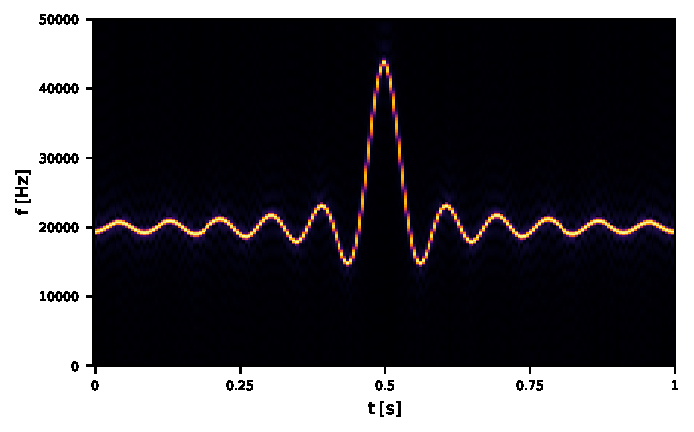
\includegraphics{papers/sonogramm/images/fm_sono_windows.pdf}
    \caption{Spektrogramm eines Frequenzmodulierten Sinus cardinalis.
    \label{sonogramm:fmsono}
    }
\end{figure}
TODO Abbildung
